
%%%%%%%% ICML 2018 EXAMPLE LATEX SUBMISSION FILE %%%%%%%%%%%%%%%%%

\documentclass{article}

% Recommended, but optional, packages for figures and better typesetting:
\usepackage{microtype}
\usepackage{graphicx}
\usepackage{subfigure}
\usepackage{booktabs} % for professional tables

% hyperref makes hyperlinks in the resulting PDF.
% If your build breaks (sometimes temporarily if a hyperlink spans a page)
% please comment out the following usepackage line and replace
% \usepackage{icml2018} with \usepackage[nohyperref]{icml2018} above.
\usepackage{hyperref}

% Attempt to make hyperref and algorithmic work together better:
\newcommand{\theHalgorithm}{\arabic{algorithm}}

\newcommand{\system}{EC2.0~}

% Use the following line for the initial blind version submitted for review:
\usepackage{icml2018}


\usepackage{hyperref}       % hyperlinks
\usepackage{url}            % simple URL typesetting
\usepackage{booktabs}       % professional-quality tables
\usepackage{amsfonts}       % blackboard math symbols
\usepackage{nicefrac}       % compact symbols for 1/2, etc.
\usepackage{microtype}      % microtypography

\usepackage{listings}
\usepackage{amsthm}
% use Times
\usepackage{times}
% For figures
\usepackage{graphicx} % more modern
%\usepackage{epsfig} % less modern
\usepackage{subfig} 
\usepackage{fancyvrb}


\usepackage{caption}
\usepackage{subcaption}

\fvset{fontsize=\footnotesize}

\usepackage{amssymb}
\usepackage{listings}
\usepackage{wrapfig}
\usepackage{tabularx}


\usepackage{verbatim}
 \usepackage{booktabs}
 % For algorithms
\usepackage{algorithm}
\usepackage{algorithmic}
\usepackage{tikz}
\usetikzlibrary{fit,bayesnet}
%\usetikzlibrary{arrows.meta}
\usetikzlibrary{positioning}
%\usetikzlibrary{decorations.text,decorations.pathreplacing}
%\usetikzlibrary{decorations.pathmorphing}
\usepackage{dsfont}
\usepackage{amsmath}
\usepackage{hyperref}
\DeclareMathOperator*{\argmin}{arg\,min} % thin space, limits underneath in displays
\DeclareMathOperator*{\argmax}{arg\,max} % thin space, limits underneath in displays
\DeclareMathOperator{\argmin}{argmin} % no space, limits underneath in displays



% Packages hyperref and algorithmic misbehave sometimes.  We can fix
% this with the following command.

\newcommand{\Expect}{\mathds{E}} %{{\rm I\kern-.3em E}}
\newcommand{\indicator}{\mathds{1}} %{{\rm I\kern-.3em E}}
\newcommand{\expect}{\mathds{E}} %{{\rm I\kern-.3em E}}
\newcommand{\probability}{\mathds{P}} %{{\rm I\kern-.3em P}}



% If accepted, instead use the following line for the camera-ready submission:
%\usepackage[accepted]{icml2018}

% The \icmltitle you define below is probably too long as a header.
% Therefore, a short form for the running title is supplied here:
\icmltitlerunning{Inducing Domain Specific Languages for Bayesian Program Learning}

\begin{document}

\twocolumn[
\icmltitle{Inducing Domain Specific Languages for Bayesian Program Learning}

% It is OKAY to include author information, even for blind
% submissions: the style file will automatically remove it for you
% unless you've provided the [accepted] option to the icml2018
% package.

% List of affiliations: The first argument should be a (short)
% identifier you will use later to specify author affiliations
% Academic affiliations should list Department, University, City, Region, Country
% Industry affiliations should list Company, City, Region, Country

% You can specify symbols, otherwise they are numbered in order.
% Ideally, you should not use this facility. Affiliations will be numbered
% in order of appearance and this is the preferred way.
\icmlsetsymbol{equal}{*}

\begin{icmlauthorlist}
\icmlauthor{Aeiau Zzzz}{equal,to}
\icmlauthor{Bauiu C.~Yyyy}{equal,to,goo}
\icmlauthor{Cieua Vvvvv}{goo}
\icmlauthor{Iaesut Saoeu}{ed}
\icmlauthor{Fiuea Rrrr}{to}
\icmlauthor{Tateu H.~Yasehe}{ed,to,goo}
\icmlauthor{Aaoeu Iasoh}{goo}
\icmlauthor{Buiui Eueu}{ed}
\icmlauthor{Aeuia Zzzz}{ed}
\icmlauthor{Bieea C.~Yyyy}{to,goo}
\icmlauthor{Teoau Xxxx}{ed}
\icmlauthor{Eee Pppp}{ed}
\end{icmlauthorlist}

\icmlaffiliation{to}{Department of Computation, University of Torontoland, Torontoland, Canada}
\icmlaffiliation{goo}{Googol ShallowMind, New London, Michigan, USA}
\icmlaffiliation{ed}{School of Computation, University of Edenborrow, Edenborrow, United Kingdom}

\icmlcorrespondingauthor{Cieua Vvvvv}{c.vvvvv@googol.com}
\icmlcorrespondingauthor{Eee Pppp}{ep@eden.co.uk}

% You may provide any keywords that you
% find helpful for describing your paper; these are used to populate
% the "keywords" metadata in the PDF but will not be shown in the document
\icmlkeywords{Machine Learning, ICML}

\vskip 0.3in
]

% this must go after the closing bracket ] following \twocolumn[ ...

% This command actually creates the footnote in the first column
% listing the affiliations and the copyright notice.
% The command takes one argument, which is text to display at the start of the footnote.
% The \icmlEqualContribution command is standard text for equal contribution.
% Remove it (just {}) if you do not need this facility.

%\printAffiliationsAndNotice{}  % leave blank if no need to mention equal contribution
\printAffiliationsAndNotice{\icmlEqualContribution} % otherwise use the standard text.

\begin{abstract}
This document provides a basic paper template and submission guidelines.
Abstracts must be a single paragraph, ideally between 4--6 sentences long.
Gross violations will trigger corrections at the camera-ready phase.
\end{abstract}

\section{Introduction}

Imagine an agent faced with a suite of new problems totally different
from anything it has seen before. It has at its disposal a basic set
of primitive actions it can compose to build solutions to these problems, but
it is no idea what kinds of primitives are appropriate for which
problems nor does it know the higher-level vocabulary in
which solutions are best expressed.
How can our agent get off the ground?

The AI and machine learning literature contains two broad takes on this problem.
The first take is that the agent should come up with a better representation of the space of solutions,
for example, by inventing new primitive actions: see \emph{options} in reinforcement learning~\cite{stolle2002learning}, the EC algorithm in program synthesis~\cite{Dechter:2013:BLV:2540128.2540316}, or predicate invention in inductive logic programming~\cite{muggleton2015meta}.
The second take is that the agent should learn a discriminative model mapping problems to a distribution over solutions: for example, policy gradient methods in reinforcement learning or neural models of program synthesis~\cite{devlin2017robustfill,balog2016deepcoder}.
Our contribution is a general algorithm for fusing these two takes on the problem:
we propose jointly inducing a representation language, called a \emph{Domain Specific Language} (DSL),
alongside a bottom-up discriminative model that regresses from problems to solutions.
We evaluate our algorithm on four domains:
building Boolean circuits; symbolic regression; FlashFill-style~\cite{gulwani2011automating} string processing problems; and Lisp-style programming problems.
We show that \system can construct a set of basis primitives suitable for discovering solutions in each of these domains

We cast these problems as \emph{Bayesian Program
  Learning} (BPL; see~\citep{lake2013one,ellis2016sampling,DBLP:conf/icml/LiangJK10}),
where the goal is to infer from an observation $x$ a posterior distribution over programs, $\probability[p|x]$.
A DSL $\mathcal{D}$ specifies the vocabulary in which programs $p$ are written.
We equip our DSLs with a \emph{weight vector} $\theta$; together, $(\mathcal{D},\theta)$
define a probabilistic generative model over programs, $\probability[p|\mathcal{D},\theta]$.
In this BPL setting, $\probability[p|x]\propto \probability[x|p]\probability[p|\mathcal{D},\theta]$,
where the likelihood $\probability[x|p]$ is domain-dependent.
The solid lines in Fig.~\ref{graphicalModel} the diagram this generative model.
Alongside this generative model,
we infer a bottom-up recognition model, $q(x)$, which is a neural network that regresses from observations to a distribution over programs.

Our key observation is that the generative and recognition models can bootstrap off of each other,
greatly increasing the tractability of BPL.


\begin{figure}
  \begin{tikzpicture}
  
  \node[latent] at (1,3) (d){$\mathcal{D}$};
  \node[latent] at (2.5,3) (t){$\theta$};
  \node[latent] at (1,1.5) (z){$p$};
  \node[latent] at (2.5,1.5) (tx){$\theta_x$};
  \node[obs] at (1,0) (x) {$x$};
  \edge {z}{x};
  \edge {d,t}{z};
  \plate {}{(tx)(z)(x)}{$N$};
  \draw [->,dashed] (x.east) to[out = 0,in = -90] node[fill = white]{$q(x)$} (tx.south);
  \draw [->,dashed] (d.west) to[out = 180,in = 180] (z.west);
  \draw [->,dashed] (tx.west) -- (z.east);
  \end{tikzpicture}
  \caption{DSL $\mathcal{D}$ generates programs $p$ by sampling DSL primitives with probabilities $\theta$ (Algorithm~\ref{programGenerativeModel}). We observe program outputs $x$. A neural network $q(\cdot )$ called the \emph{recognition model} regresses from program outputs to a distribution over programs ($\theta_x = q(x)$). Solid arrows correspond to the top-down generative model. Dashed arrows correspond to the bottom-up recognition model.}\label{graphicalModel}
\end{figure}

\section{Program Representation}
We choose to represent programs using $\lambda$-calculus~\cite{pierce}.
A $\lambda$-calculus expression is either:
\\\noindent A \emph{primitive}, like the number 5 or
  the function \texttt{sum}.
\\\noindent A \emph{variable}, like $x$, $y$, $z$
\\\noindent A $\lambda$\emph{-abstraction}, which creates a new function. $\lambda$-abstractions have a variable and a body. The body is a $\lambda$-calculus expression. Abstractions are written as $\lambda \text{var}. \text{body}$.
\\\noindent An \emph{application} of a function to an argument. Both the function and the argument are $\lambda$-calculus expressions. The application of the function $f$ to the argument $x$ is written as $f\; x$.

For example, the function which squares the logarithm of a number is
$\lambda x.\text{\texttt{square}} (\text{\texttt{log} } x)$, and the identity function $f(x) = x$ is $\lambda x.x$. The
$\lambda$-calculus serves as a spartan but expressive Turing complete
program representation, and distills the essential features of functional languages like Lisp.

However, many $\lambda$-calculus expressions correspond to ill-typed programs, such as the program that takes the logarithm of the Boolean \texttt{true} (i.e., \texttt{log true}) or which applies the number five to the identity function
(i.e., $5 \; (\lambda x.x)$).
We use a well-established typing system for $\lambda$-calculus called \emph{Hindley-Milner typing}~\cite{pierce}, which is used in programming languages like OCaml.
The purpose of the typing system is to ensure that our programs never call a function with a type it is not expecting (like trying to take the logarithm of \texttt{true}).
Hindley-Milner has two important features:
Feature 1: It supports \emph{parametric polymorphism}: meaning that types can have variables in them, called \emph{type variables}. Lowercase Greek letters are conventionally used for  type variables.
For example, the type of the identity function is $\alpha\to\alpha$, meaning it takes something of type $\alpha$ and return something of type $\alpha$. A function that returns the first element of a list has the type $\texttt{list}(\alpha)\to\alpha$. Type variables are not the same has variables introduced by $\lambda$-abstractions.
Feature 2: Remarkably, there is a  simple algorithm for automatically inferring the polymorphic Hindley-Milner type of a $\lambda$-calculus expression~\cite{damas1982principal}.
A detailed exposition of Hindley-Milner is beyond the scope of this work.

%% \begin{figure}
%%   \begin{align}
%%     \text{primitive types} & 
%%     \end{align}
%%   \end{figure}



\section{Experiments}

\begin{figure}
  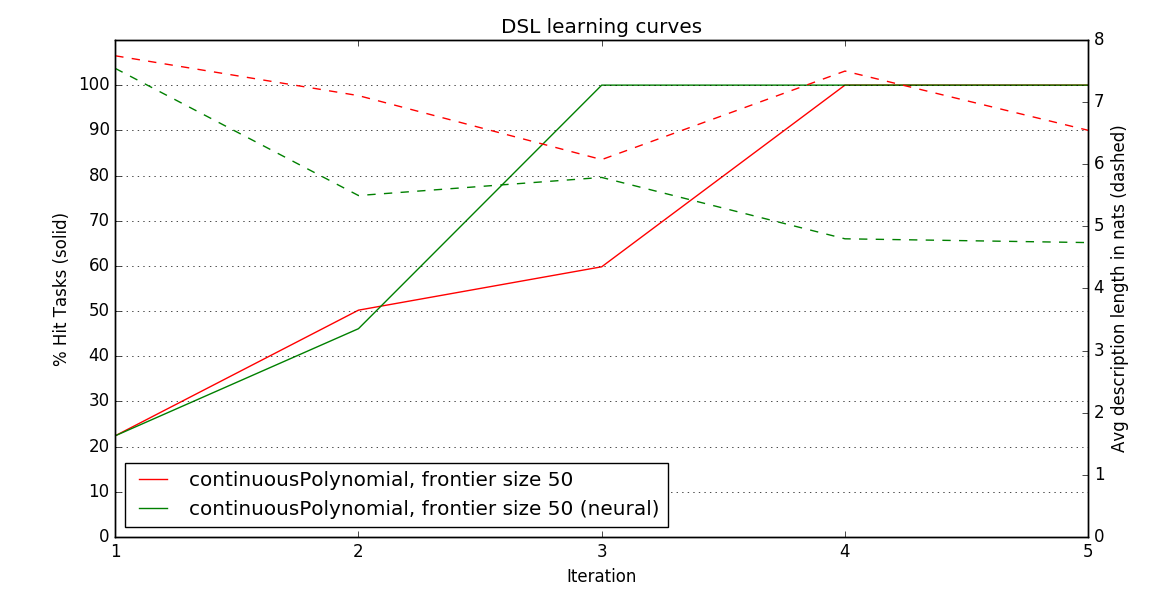
\includegraphics[width = 9cm]{figures/polynomial.png}
  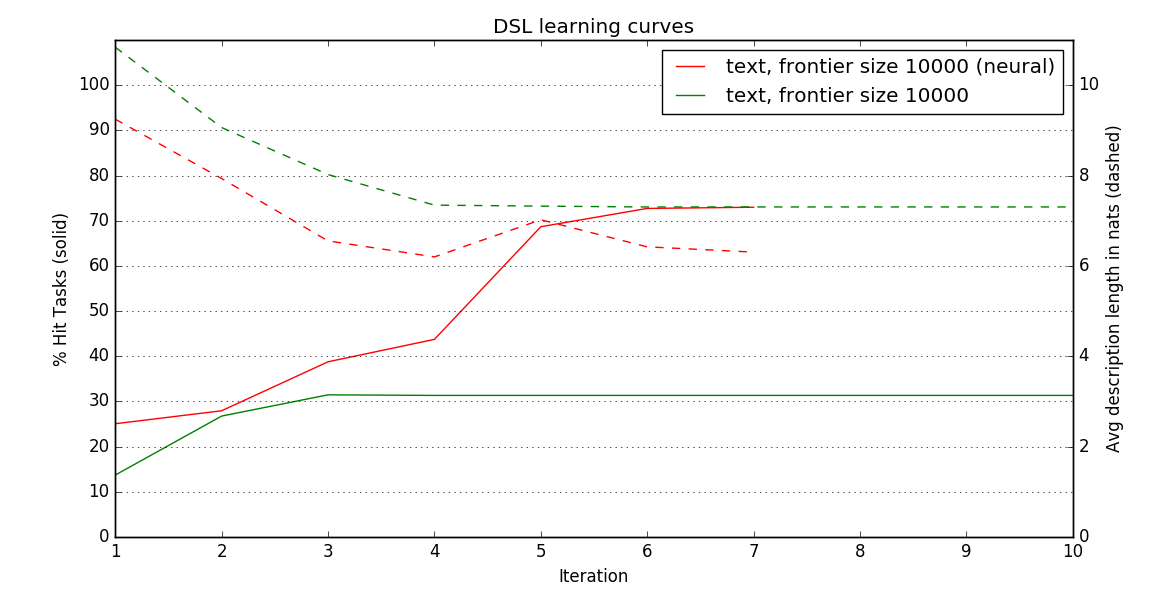
\includegraphics[width = 9cm]{figures/text.png}
  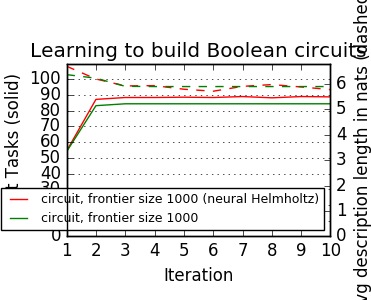
\includegraphics[width = \columnwidth]{figures/circuit.png} 
\end{figure}

\section{Model}



\section{Implementation}

\begin{algorithm}[tb]
   \caption{Generative model over programs}
   \label{programGenerativeModel}
   \begin{algorithmic}
     \STATE \textbf{function} sample$(\mathcal{D}, \theta, \mathcal{E}, \tau)$:
  \STATE {\bfseries Input:} DSL $\mathcal{D}$, weight vector $\theta$, environment $\mathcal{E}$, type $\tau$
  \STATE \textbf{Output:} a program whose type unifies with $\tau$
  \IF{$\tau = \alpha\to\beta$}
  \STATE var $\gets$ an unused variable name
  \STATE body $\sim$ sample$(\mathcal{D},\theta,[\text{var}:\alpha]+\mathcal{E},\beta)$
   \STATE \textbf{return} $\lambda \text{var}.$ body
   \ENDIF
   %   \ELSE
   \STATE\begin{align*}     \text{primitives} \gets\{p | &p:\alpha\to\cdots\to\beta \in \mathcal{D}\cup\mathcal{E}\\     &\text{if canUnify}(\tau,\beta) \}     \end{align*}
   
   \STATE Sample $e\sim \text{primitives}$, w.p. $\propto\theta_e$ if $e\in \mathcal{D}$ and w.p. $\propto\frac{\theta_{var}}{|\text{variables}|}$ if $e\in \mathcal{E}$
   \STATE Let $e:\alpha_1\to\alpha_2\to\cdots\to \alpha_K\to\beta$. Unify $\tau$ with $\beta$.
%   \STATE unify$(\tau,\beta)$
   \FOR{$k=1$ {\bfseries to} $K$}
 \STATE $a_k\sim\text{sample}(\mathcal{D},\theta,\mathcal{E},\alpha_k)$
 \ENDFOR
 \STATE \textbf{return} $e(a_1, a_2, \cdots, a_K)$
 %  \UNTIL{$noChange$ is $true$}
\end{algorithmic}
\end{algorithm}

\begin{algorithm}[tb]
   \caption{DSL Learner}
   \label{mainAlgorithm}
   \begin{algorithmic}
     \STATE {\bfseries Input:} Initial DSL $\mathcal{D}$, set of tasks $X$, iterations $I$
     \STATE \textbf{Hyperparameters:} Frontier size $F$
     \STATE \textbf{Output:} DSL $\mathcal{D}$, weight vector $\theta$, bottom-up recognition model $q(\cdot)$
     \STATE Initialize $\mathcal{D}_0\gets \mathcal{D}$, $\theta_0\gets \text{uniform}$, $q_0(\cdot ) = \theta_0$
     \FOR{$i=1$ {\bfseries to} $I$}
     \FOR{$x:\tau\in X$}
     \STATE  $\mathcal{F}_x\gets \{z| z\in \text{enumerate}(\mathcal{D}_{i - 1},q_{i - 1}(x),F)\cup\text{enumerate}(\mathcal{D}_{i - 1},\theta_{i - 1},F) \text{ if }\probability[x|z] > 0\}$
     \ENDFOR
     \STATE $\mathcal{D}_i,\theta_i\gets $induceGrammar$(\{\mathcal{F}_x\}_{x\in X})$
     \STATE Define $Q_x(z) \propto \begin{cases}
       \probability[x|z]\probability[z|\mathcal{D}_i,\theta_i]&x\in \mathcal{F}_x\\
       0&x\not \in \mathcal{F}_x
     \end{cases}$
     \STATE $q_i\gets \argmin_q \sum_{x\in X}\text{KL}(Q_x(\cdot )||\probability[\cdot |\mathcal{D}_i,q(x)])$
      \ENDFOR
 \STATE \textbf{return} $\mathcal{D}^I,\theta^I,q^I$
\end{algorithmic}
\end{algorithm}

\begin{algorithm}[tb]
   \caption{Grammar Induction Algorithm}
   \label{grammarInductionAlgorithm}
   \begin{algorithmic}
     \STATE {\bfseries Input:} Set of frontiers $\{\mathcal{F}_x\}$
     \STATE \textbf{Hyperparameters:} Pseudocounts $\alpha$, regularization parameter $\lambda$, AIC coefficient $a$
     \STATE \textbf{Output:} DSL $\mathcal{D}$, weight vector $\theta$
     \STATE Define $\log \probability[\mathcal{D}]\stackrel{+}{ = } -\lambda\sum_{p\in \mathcal{D}} \text{size}(p)$
     \STATE Define $L(\mathcal{D},\theta) =  \prod_x \sum_{z\in \mathcal{F}_x} \probability[z|\mathcal{D},\theta]$
     \STATE Define $\theta^*(\mathcal{D}) = \argmax_\theta \text{Dir}(\theta|\alpha) L(\mathcal{D},\theta)$
     \STATE Define $\text{score}(\mathcal{D}) = \log \probability[\mathcal{D}] + L(\mathcal{D},\theta^*) - a|\mathcal{D}|$
     \STATE $\mathcal{D}\gets$ every primitive in $\{\mathcal{F}_x\}$
     \WHILE {true}
     \STATE N $\gets \{\mathcal{D}\cup \{s\} | x\in X, z\in \mathcal{F}_x, s\text{ a subtree of }z\}$
     \STATE $\mathcal{D}'\gets \argmax_{\mathcal{D}'\in N}\text{score}(\mathcal{D}') $
     \IF{$\text{score}(\mathcal{D}') > \text{score}(\mathcal{D})$}
     \STATE $\mathcal{D}\gets\mathcal{D}'$
     \ELSE
     \STATE\textbf{return} $\mathcal{D},\theta^*(\mathcal{D})$
     \ENDIF
     \ENDWHILE
   \end{algorithmic}
\end{algorithm}

\section{Estimating the grammar parameters}

I justify this estimator by proving that it maximizes a lower bound on the log likelihood of the data. Writing $L$ for the log likelihood, $\theta$ for the parameters of the grammar, $N$ for the number of random choices, $A$ to range over the alternative choices for a random variable, $c(x)$ to mean the number of times that primitive $x$ was used, and $a(x) = \sum_A \indicator [x\in A]$ to mean the number of times that primitive $x$ could have been used:
\begin{align}
  L& = \sum_x c(x)\log \theta_x - \sum_A \log \sum_{x\in A}\theta_x\\
  & = \sum_x c(x)\log \theta_x - N\expect_A \log \sum_{x\in A}\theta_x\\
  &\geq\sum_x c(x)\log \theta_x - N \log \expect_A \sum_{x\in A}\theta_x\text{, Jensen's inequality}\\
  & = \sum_x c(x)\log \theta_x - N \log \frac{1}{N}\sum_A \sum_{x} \indicator [x\in A]\theta_x\\
  & \stackrel{+}{=} \sum_x c(x)\log \theta_x - N \log \sum_x a(x)\theta_x.
\end{align}
Differentiate with respect to $\theta_x$ and set to zero:
\begin{align}
  \frac{c(x)}{\theta_x} &= N\frac{a(x)}{\sum_y a(y)\theta_y}
\end{align}
This equality holds if $\theta_x = c(x)/a(x)$:
\begin{align}
  \frac{c(x)}{\theta_x} &= a(x).\\
N\frac{a(x)}{\sum_y a(y)\theta_y}& = N\frac{a(x)}{\sum_y c(y)}   = N\frac{a(x)}{N} = a(x).
\end{align}
If this equality holds then $\theta_x \propto c(x)/a(x)$:
\begin{align}
  \theta_x = \frac{c(x)}{a(x)}\times \underbrace{\frac{\sum_y a(y)\theta_y}{N}}_{\text{Independent of $x$}}.
\end{align}

Now what we are actually after is the parameters that maximize the joint log probability of the data+parameters, which I will write $J$:
\begin{align}
  J& = L + \log \text{D}(\theta|\alpha)\\
  &\stackrel{+}{\geq } \sum_x c(x)\log \theta_x - N \log \sum_x a(x)\theta_x  + \sum_x(\alpha_x - 1)\log \theta_x\\
  & = \sum_x (c(x) + \alpha_x - 1)\log \theta_x -  N \log \sum_x a(x)\theta_x
\end{align}
So you add the pseudocounts to the \emph{counts} ($c(x)$), but not to the \emph{possible counts} ($a(x)$).


\bibliography{main}
\bibliographystyle{icml2018}

\end{document}


% This document was modified from the file originally made available by
% Pat Langley and Andrea Danyluk for ICML-2K. This version was created
% by Iain Murray in 2018. It was modified from a version from Dan Roy in
% 2017, which was based on a version from Lise Getoor and Tobias
% Scheffer, which was slightly modified from the 2010 version by
% Thorsten Joachims & Johannes Fuernkranz, slightly modified from the
% 2009 version by Kiri Wagstaff and Sam Roweis's 2008 version, which is
% slightly modified from Prasad Tadepalli's 2007 version which is a
% lightly changed version of the previous year's version by Andrew
% Moore, which was in turn edited from those of Kristian Kersting and
% Codrina Lauth. Alex Smola contributed to the algorithmic style files.
